\documentclass[border=0.15cm]{standalone}
\usepackage{tikz}
\usetikzlibrary{automata, arrows.meta, positioning}

\begin{document}
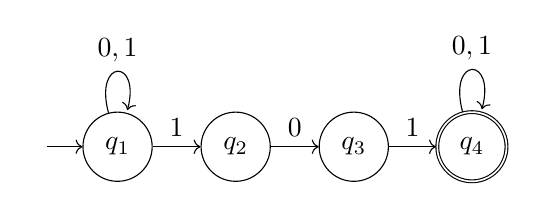
\begin{tikzpicture}
    every initial by arrow/.style = {-To},
    every loop/.style = {-To}]
    % \draw [help lines] (-1,-1) grid (5,1);
    \node (q1) [state, 
        initial, 
        initial text={}] at (0,0) {$q_{1}$};
    \node (q2) [state] at (1.5,0) {$q_{2}$};
    \node (q3) [state] at (3.0,0) {$q_{3}$};
    \node (q4) [state, 
        accepting] at (4.5,0) {$q_{4}$};
    
    \path [-To]
        (q1) edge node [above] {$1$} (q2)
        (q2) edge node [above] {$0$} (q3)
        (q3) edge node [above] {$1$} (q4)
        (q1) edge [loop above] node {$0,1$} ()
        (q4) edge [loop above] node {$0,1$} ();
\end{tikzpicture}
\end{document}